

\section{Ethernet 1 (LAN, Grundlagen)}


\subsection{Topologien}

{
    \begin{tikzpicture}
        \node [examplebox] (box){
            \begin{minipage}{0.3\textwidth}
                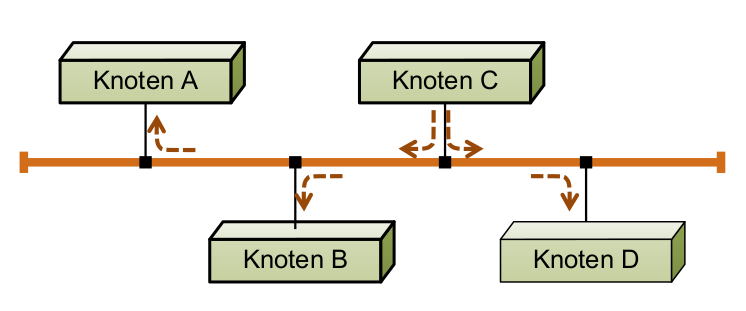
\includegraphics[scale=.15]{img/bus.png}
                {  \scriptsize
                    \begin{itemize}[noitemsep]
                        \item Alle Stationen: sind passiv angeschlossen, horchen Leitung permanent ab, werden aktiv, wenn sie etwas senden wollen
                        \item Taktrückgewinnung erlauben, um eine separate Taktleitung einzusparen
                        \item Empfänger erkennt anhand einer Adresse,
                              ob die Daten für ihn relevant sind
                    \end{itemize}
                }
            \end{minipage}
        };
        \node[exampletitle, right=8pt] at (box.north west) {Bus};
    \end{tikzpicture}

    \begin{tikzpicture}
        \node [examplebox] (box){
            \begin{minipage}{0.3\textwidth}
                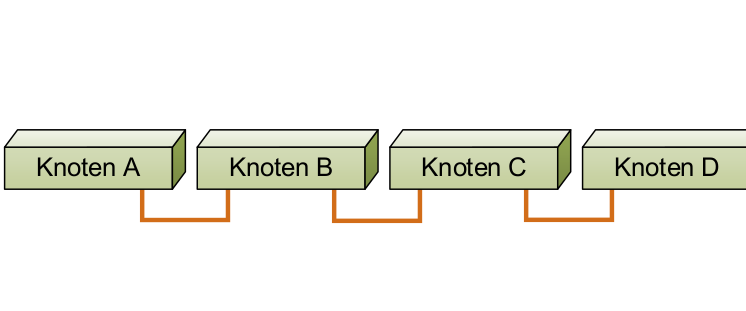
\includegraphics[scale=.15]{img/linie.png}
                {  \scriptsize  \begin{itemize}[noitemsep]
                        \item Punkt-zu-Punkt Verbindungen zwischen benachbarten Knoten
                        \item Alle Stationen müssen: Daten empfangen, Daten regenerieren, falls nötig weiterleiten
                        \item Der Ausfall einer Station führt zur
                              Segmentierung des LAN in zwei Teile
                    \end{itemize}}
            \end{minipage}
        };
        \node[exampletitle, right=8pt] at (box.north west) {Linie};
    \end{tikzpicture}

    \begin{tikzpicture}
        \node [examplebox] (box){
            \begin{minipage}{0.3\textwidth}
                \includegraphics[scale=.15]{img/Ring.png}
                {  \scriptsize  \begin{itemize}[noitemsep]
                        \item Benötigt Verfahren zur Verhinderung von "endlosem Kreisverkehr"
                        \item Gewisse Redundanz: beim Ausfall einer Station kann immer noch jede Station erreicht werden
                    \end{itemize}}
            \end{minipage}
        };
        \node[exampletitle, right=8pt] at (box.north west) {Ring};
    \end{tikzpicture}
    \vfill\null

    \begin{tikzpicture}
        \node [examplebox] (box){
            \begin{minipage}{0.3\textwidth}
                \includegraphics[scale=.15]{img/Vermascht.png}
                {  \scriptsize  \begin{itemize}[noitemsep]
                        \item Weitere Erhöhung der Redundanz:
                        \item Ausfall einer oder eventuell auch mehrerer Stationen oder Verbindungen kann toleriert werden
                        \item Zusätzliche Kosten und Aufwand, um mehrfache Lieferung von Daten zuverhindern
                    \end{itemize}}
            \end{minipage}
        };
        \node[exampletitle, right=8pt] at (box.north west) {Vermascht};
    \end{tikzpicture}


    \begin{tikzpicture}
        \node [examplebox] (box){
            \begin{minipage}{0.3\textwidth}
                \includegraphics[scale=.15]{img/Stern.png}
                {  \scriptsize  \begin{itemize}[noitemsep]
                        \item Jede Station an zentralen Verteiler (Switch/Bridge) angeschlossen
                        \item Verteiler entkoppelt Knoten elektrisch und macht LAN weniger störungsanfällig
                        \item Verteiler sendet Daten, die er von einerStation erhält, an die anderen Knoten weiter
                    \end{itemize}}
            \end{minipage}
        };
        \node[exampletitle, right=8pt] at (box.north west) {Stern};
    \end{tikzpicture}

    \begin{tikzpicture}
        \node [examplebox] (box){
            \begin{minipage}{0.3\textwidth}
                \includegraphics[scale=.15]{img/Baum.png}
                {  \scriptsize
                    \begin{itemize}[noitemsep]
                        \item Hierarchische Erweiterung der Sterntopologie
                        \item Intelligenten Switches ermöglichen einen Grossteil der Kommunikation „lokal“
                        \item Dadurch Verringerung der Last für die einzelnen Switches
                    \end{itemize}}
            \end{minipage}
        };
        \node[exampletitle, right=8pt] at (box.north west) {Baum};
    \end{tikzpicture}
    \vfill\null
}

\columnbreak
\subsection{Layer 3 Aufgaben:}
{

    \begin{itemize}[noitemsep]
        \item Netzweite Adressierung
        \item Nachführen der Routing Informationen
        \item Ermitteln des optimalen Weges
        \item Weiterleiten der Daten über den festgelegten Weg
    \end{itemize}
}




\subsection{Übertragungsarten}{
    \begin{multicols*}{2}

        \begin{tikzpicture}
            \node [examplebox] (box){
                \begin{minipage}{0.15\textwidth}
                    \includegraphics[scale=.2]{img/Unicast.png}
                    {\scriptsize
                        \begin{itemize}[noitemsep]
                            \item Genau ein, klar spezifizierter Empfänger
                            \item Frame trägt die Adresse dieses Empfängers
                            \item Analogie: Briefpost
                        \end{itemize}}
                \end{minipage}
            };
            \node[exampletitle, right=8pt] at (box.north west) {Unicast};
        \end{tikzpicture}


        \begin{tikzpicture}
            \node [examplebox] (box){
                \begin{minipage}{0.15\textwidth}
                    \includegraphics[scale=.2]{img/Multicast.png}
                    {  \scriptsize
                        \begin{itemize}[noitemsep]
                            \item Gruppe von Empfängern
                            \item Frame trägt die Multicast-Adresse der Gruppe
                            \item Analogie: Mailing-Liste
                        \end{itemize}}
                \end{minipage}
            };
            \node[exampletitle, right=8pt] at (box.north west) {Multicast};
        \end{tikzpicture}

        \begin{tikzpicture}
            \node [examplebox] (box){
                \begin{minipage}{0.15\textwidth}
                    \includegraphics[scale=.2]{img/Broadcast.png}
                    {  \scriptsize
                        \begin{itemize}[noitemsep]
                            \item An alle Knoten im LAN gerichtet
                            \item Frame trägt die Broadcast-Adresse des LAN
                            \item Analogie: Radio-Sendestation
                        \end{itemize}}
                \end{minipage}
            };
            \node[exampletitle, right=8pt] at (box.north west) {Broadcast};
        \end{tikzpicture}

    \end{multicols*}

}

\subsection{10 Mbit/s (10BASE-T) Manchester Codierung}{
    \begin{itemize}[noitemsep]
        \item Erlaubt die Taktrückgewinnung auf einfache Weise: weil Bei jedem Bit gibt es einen Signalwechsel
        \item Bandbreite von 10 MHz benötigt (also das doppelte des theoretischen Minimums)
        \item   1 positive Flanke, 0 negative Flanke
    \end{itemize}

    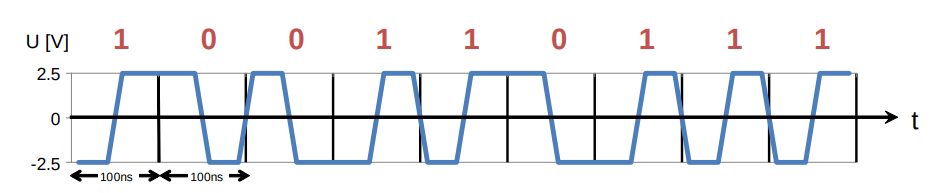
\includegraphics[scale=.275]{img/manchester.png}

}
\vfill\null
\columnbreak
\subsection{100 Mbit/s (100BASE-TX) NRZI-Codierung }{
    {  \begin{itemize}[noitemsep]
                \item NRZI-Codierung (Non Return to Zero Inverted),kombiniert mit MLT-3 (MLT-3 = Multi-Level Transmit) 125 MBaud → 1 Symbol entspricht 8 ns
                \item 4B/5B Code Leitungscodierung
                \item 4 Bits des MII (Zeichen) werden mit einem 5 Bit-Zeichen (Code Group) auf der Leitung codiert
            \end{itemize}

            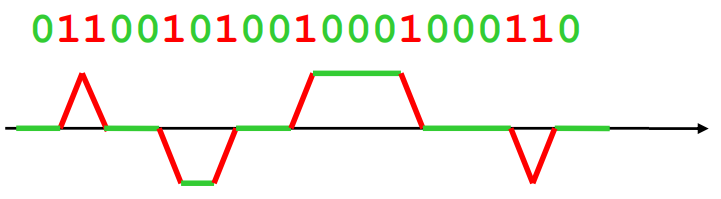
\includegraphics[scale=.275]{img/NRZI.png}

        }

}


\subsection{MAC Adressen}{
Adressierung in LANs, bestehen aus 6 Bytes \\

{Registrierung bei IEEE}

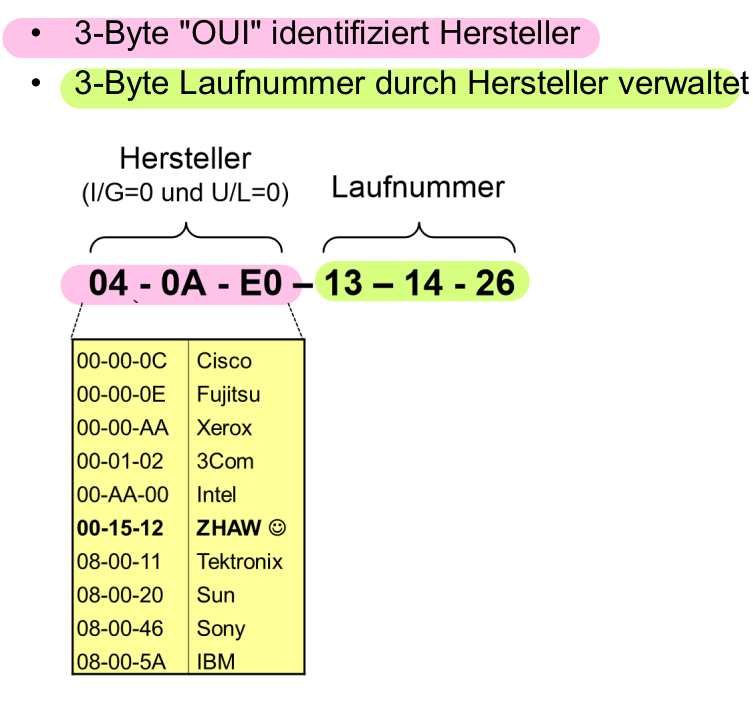
\includegraphics[scale=.25]{img/mac-1.png}

{
    {Zwei Bits klassifizieren die MAC Adresse:} \\
    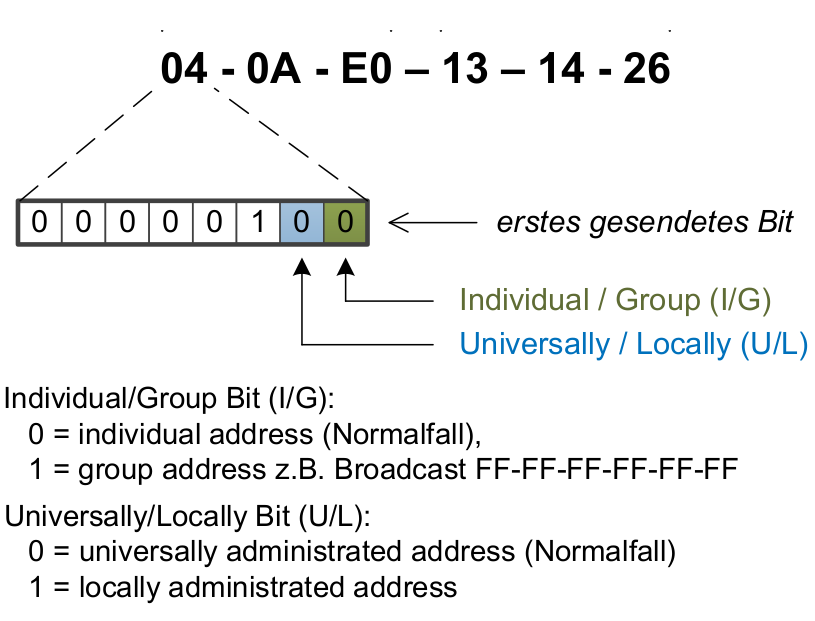
\includegraphics[scale=.25]{img/mac-2.png}
}
}


\columnbreak
\subsection{Ethernet Types:}{

    \begin{itemize}[noitemsep]
        \item 0x0800 $\to$ IPv4
        \item 0x0806 $\to$  ARP
        \item  0x8100 $\to$  VLA-tagged
        \item  0x86DD $\to$  IPv6
    \end{itemize}




}
\subsection{Switch Performance}{

    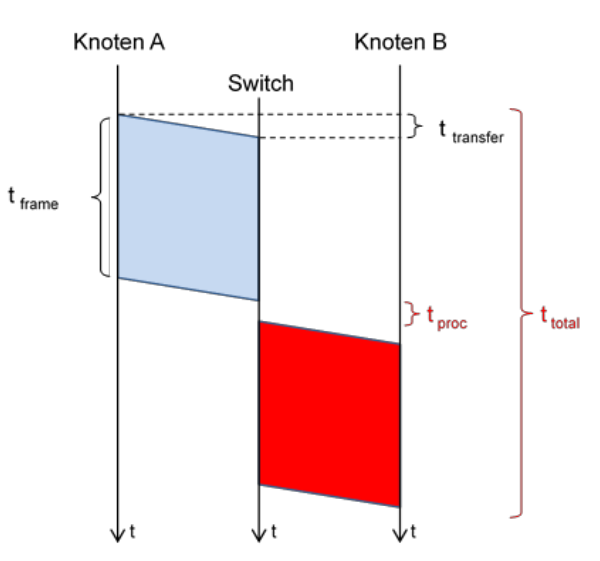
\includegraphics[scale=.3]{img/sw-perf.png}
    \\
    $$ \text{t}_\text{frame} = \frac{\text{Framesize}}{\text{Bitrate}}  $$

    $$ \text{t}_\text{delay} = \frac{\text{Framesize} \cdot 8}{\text{Bitrate}}  $$
    $$ \text{t}_\text{transfer} = \frac{\text{Leitungslänge}}{\text{Ausb. geschwindigkeit}}  $$

    Falls nur Nutzdaten angegeben:
    $$ \tiny \text{t}_\text{frame} = \frac{\text{[Data + 8 (Prä/SFD) + 12 (MACs) + 2 (Type) + 4 (FCS)]}\cdot 8}{\text{Bitrate}}  $$

}
\vfill\null
\columnbreak
\subsection{Ethernet - Frame Format}{
    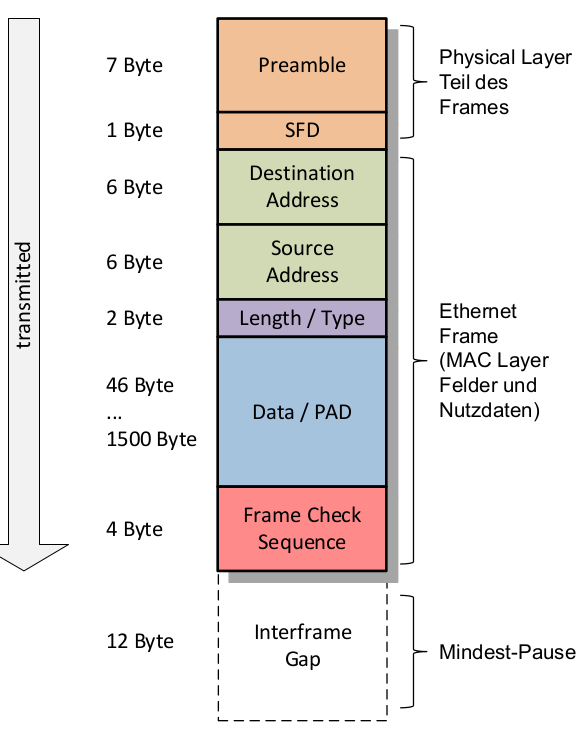
\includegraphics[scale=.275]{img/E-Frame.png}

    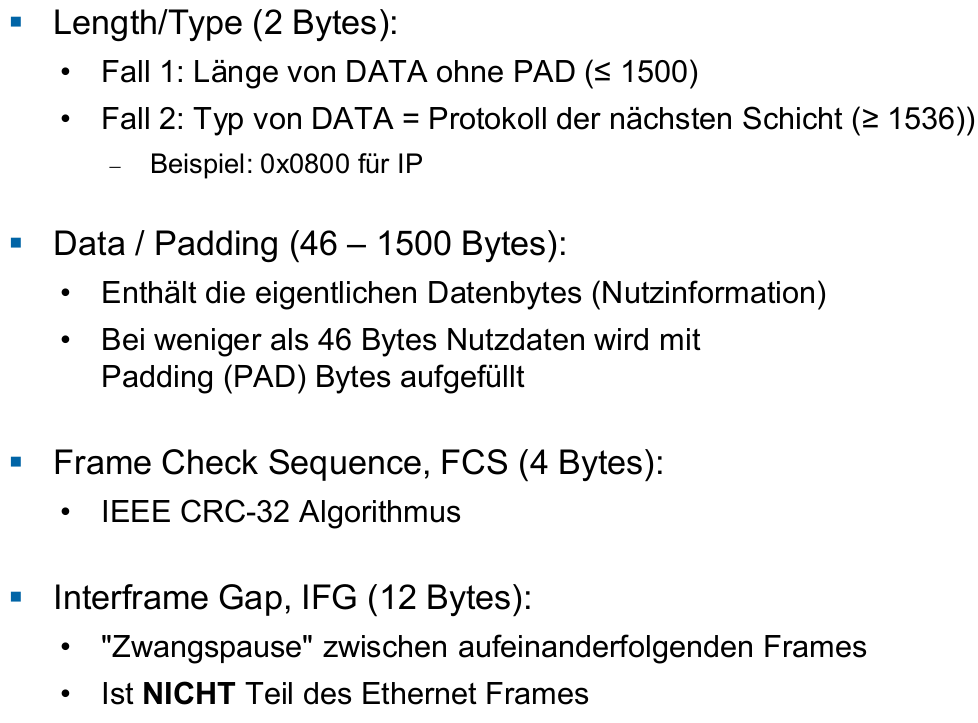
\includegraphics[scale=.275]{img/E-2.png}
}



